\Def \textbf{Геометрическая вероятность.}

Пусть $\Omega \subset \R^n$ и $p(A) = \frac{\mu(A)}{\mu(\Omega)}$

Много задач на геометрическую вероятность разобрано тут:

\url{http://www.mathprofi.ru/geometricheskoe_opredelenie_verojatnosti.html}

\textbf{Задача.}

Староста группы заметил, что семинарист приходит на занятия со случайным опозданием в пределах $15$ минут. При этом семинарист не пускает в аудиторию студентов, которые пришли после него позднее чем на $5$ минут. Староста же решил опоздать на семинар, но выбрал себе границу случайного опоздания всего в $10$ минут. Также он решила ждать семинариста не более $10$ минут после своего прихода, а если его не будет -- уйти. Какова вероятность того, что староста все же посетит семинар?

\underline{Решение}

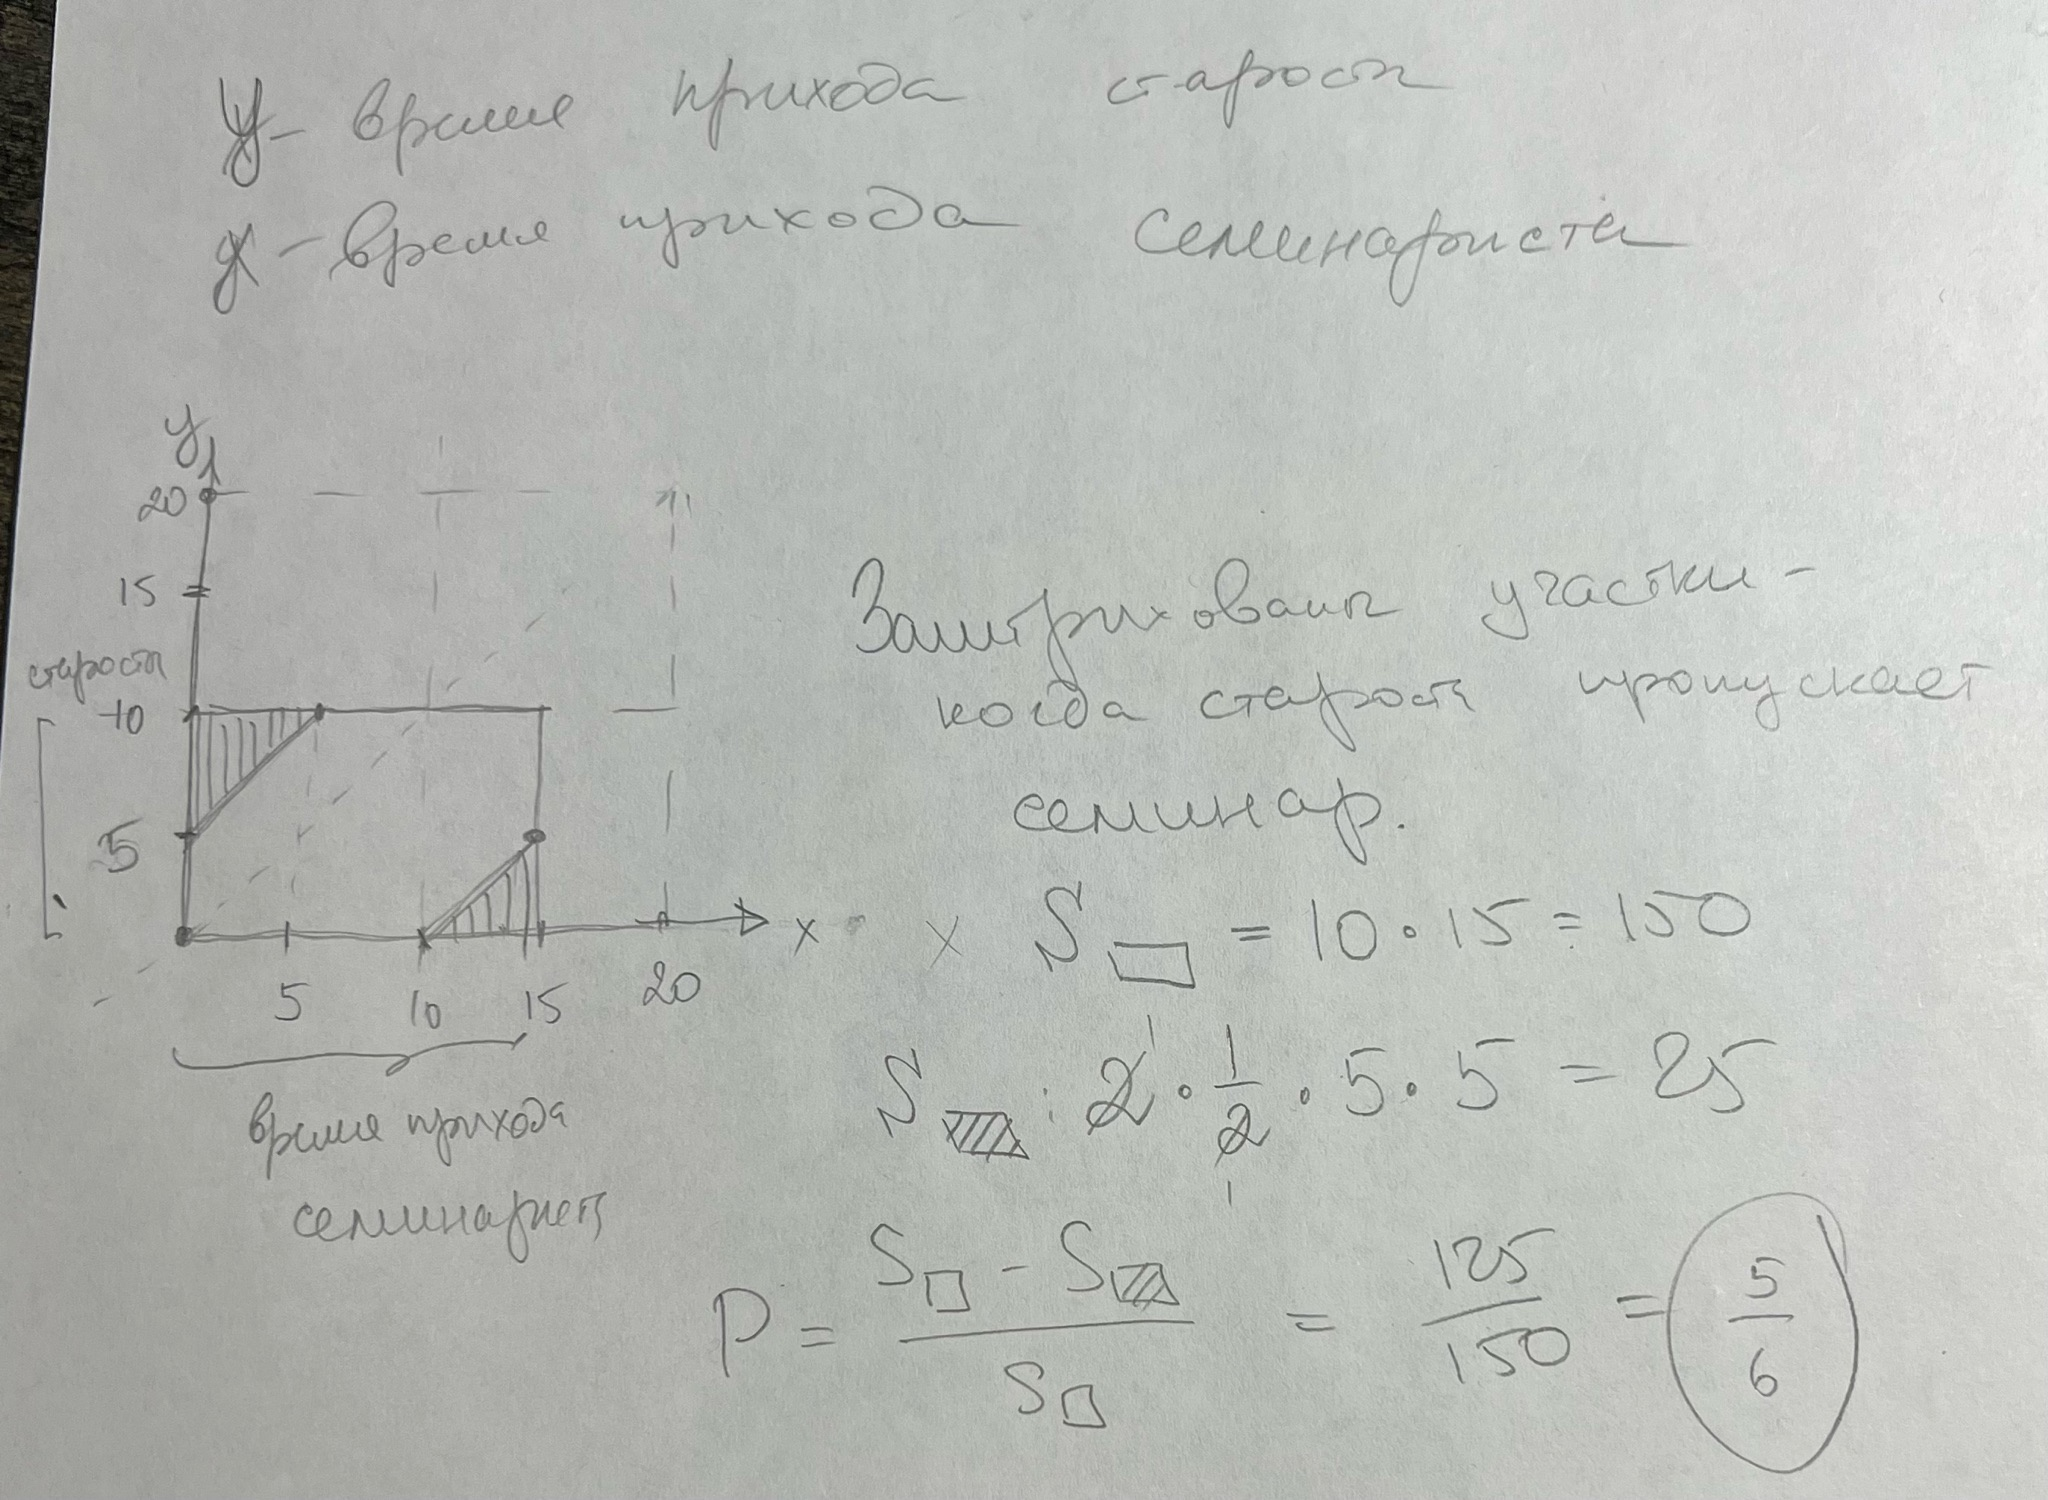
\includegraphics[width=12cm]{images/jetminded_solution.jpeg}